\section{Results}
% prec:0.154787009701     f1:0.179024390244       jac:0.0983123493169

We performed experiments to evaluate the performance of the feature classification. The experimental setup described in the previous section shows that we have many parameters that could influence the classification performance. We will therefore first show results for a certain set of parameters that performed well. In the further sections, we explore the effects of different parameters, such as different feature sets, classification algorithms, and test images.

%In this case, the classifiers were trained on section two and three and tested on section one. Furthermore, these results were obtained using synthetic oversampling using the SMOTE method.


\begin{figure}
	\centering
	\begin{tabular}{cc}
		\subfloat{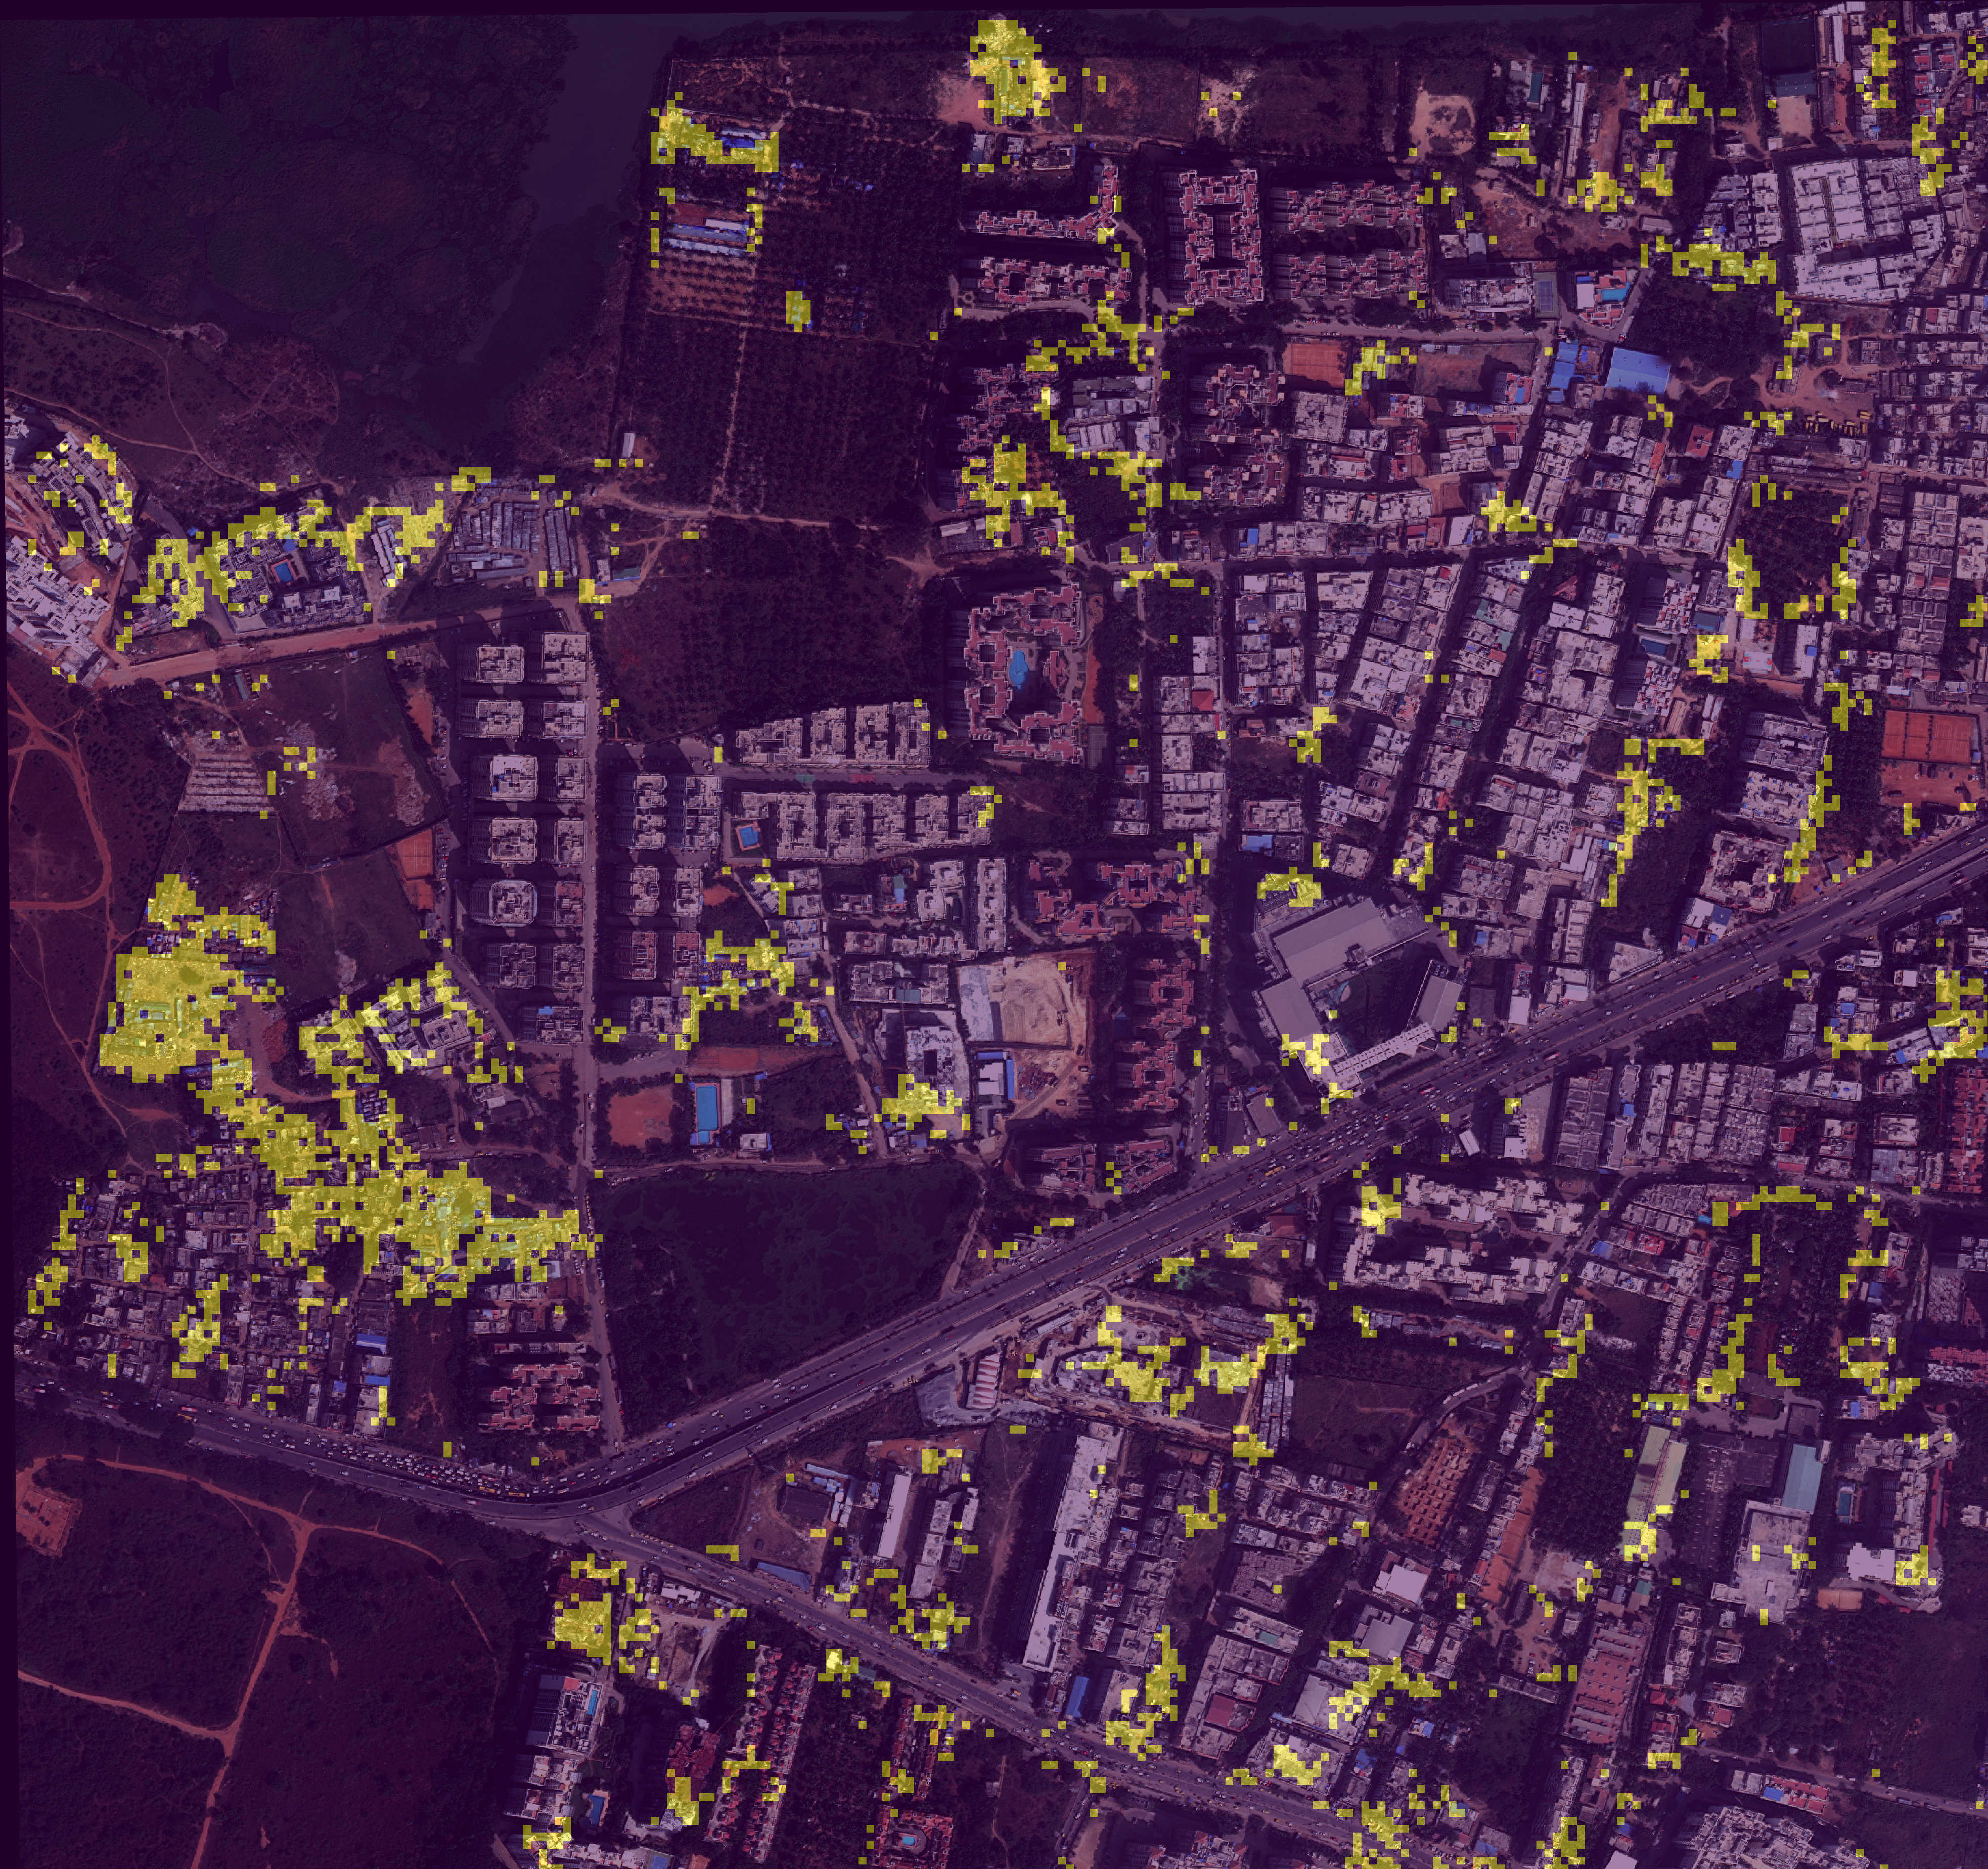
\includegraphics[width=0.5\textwidth]{images/BestOverlay}}&
		\subfloat{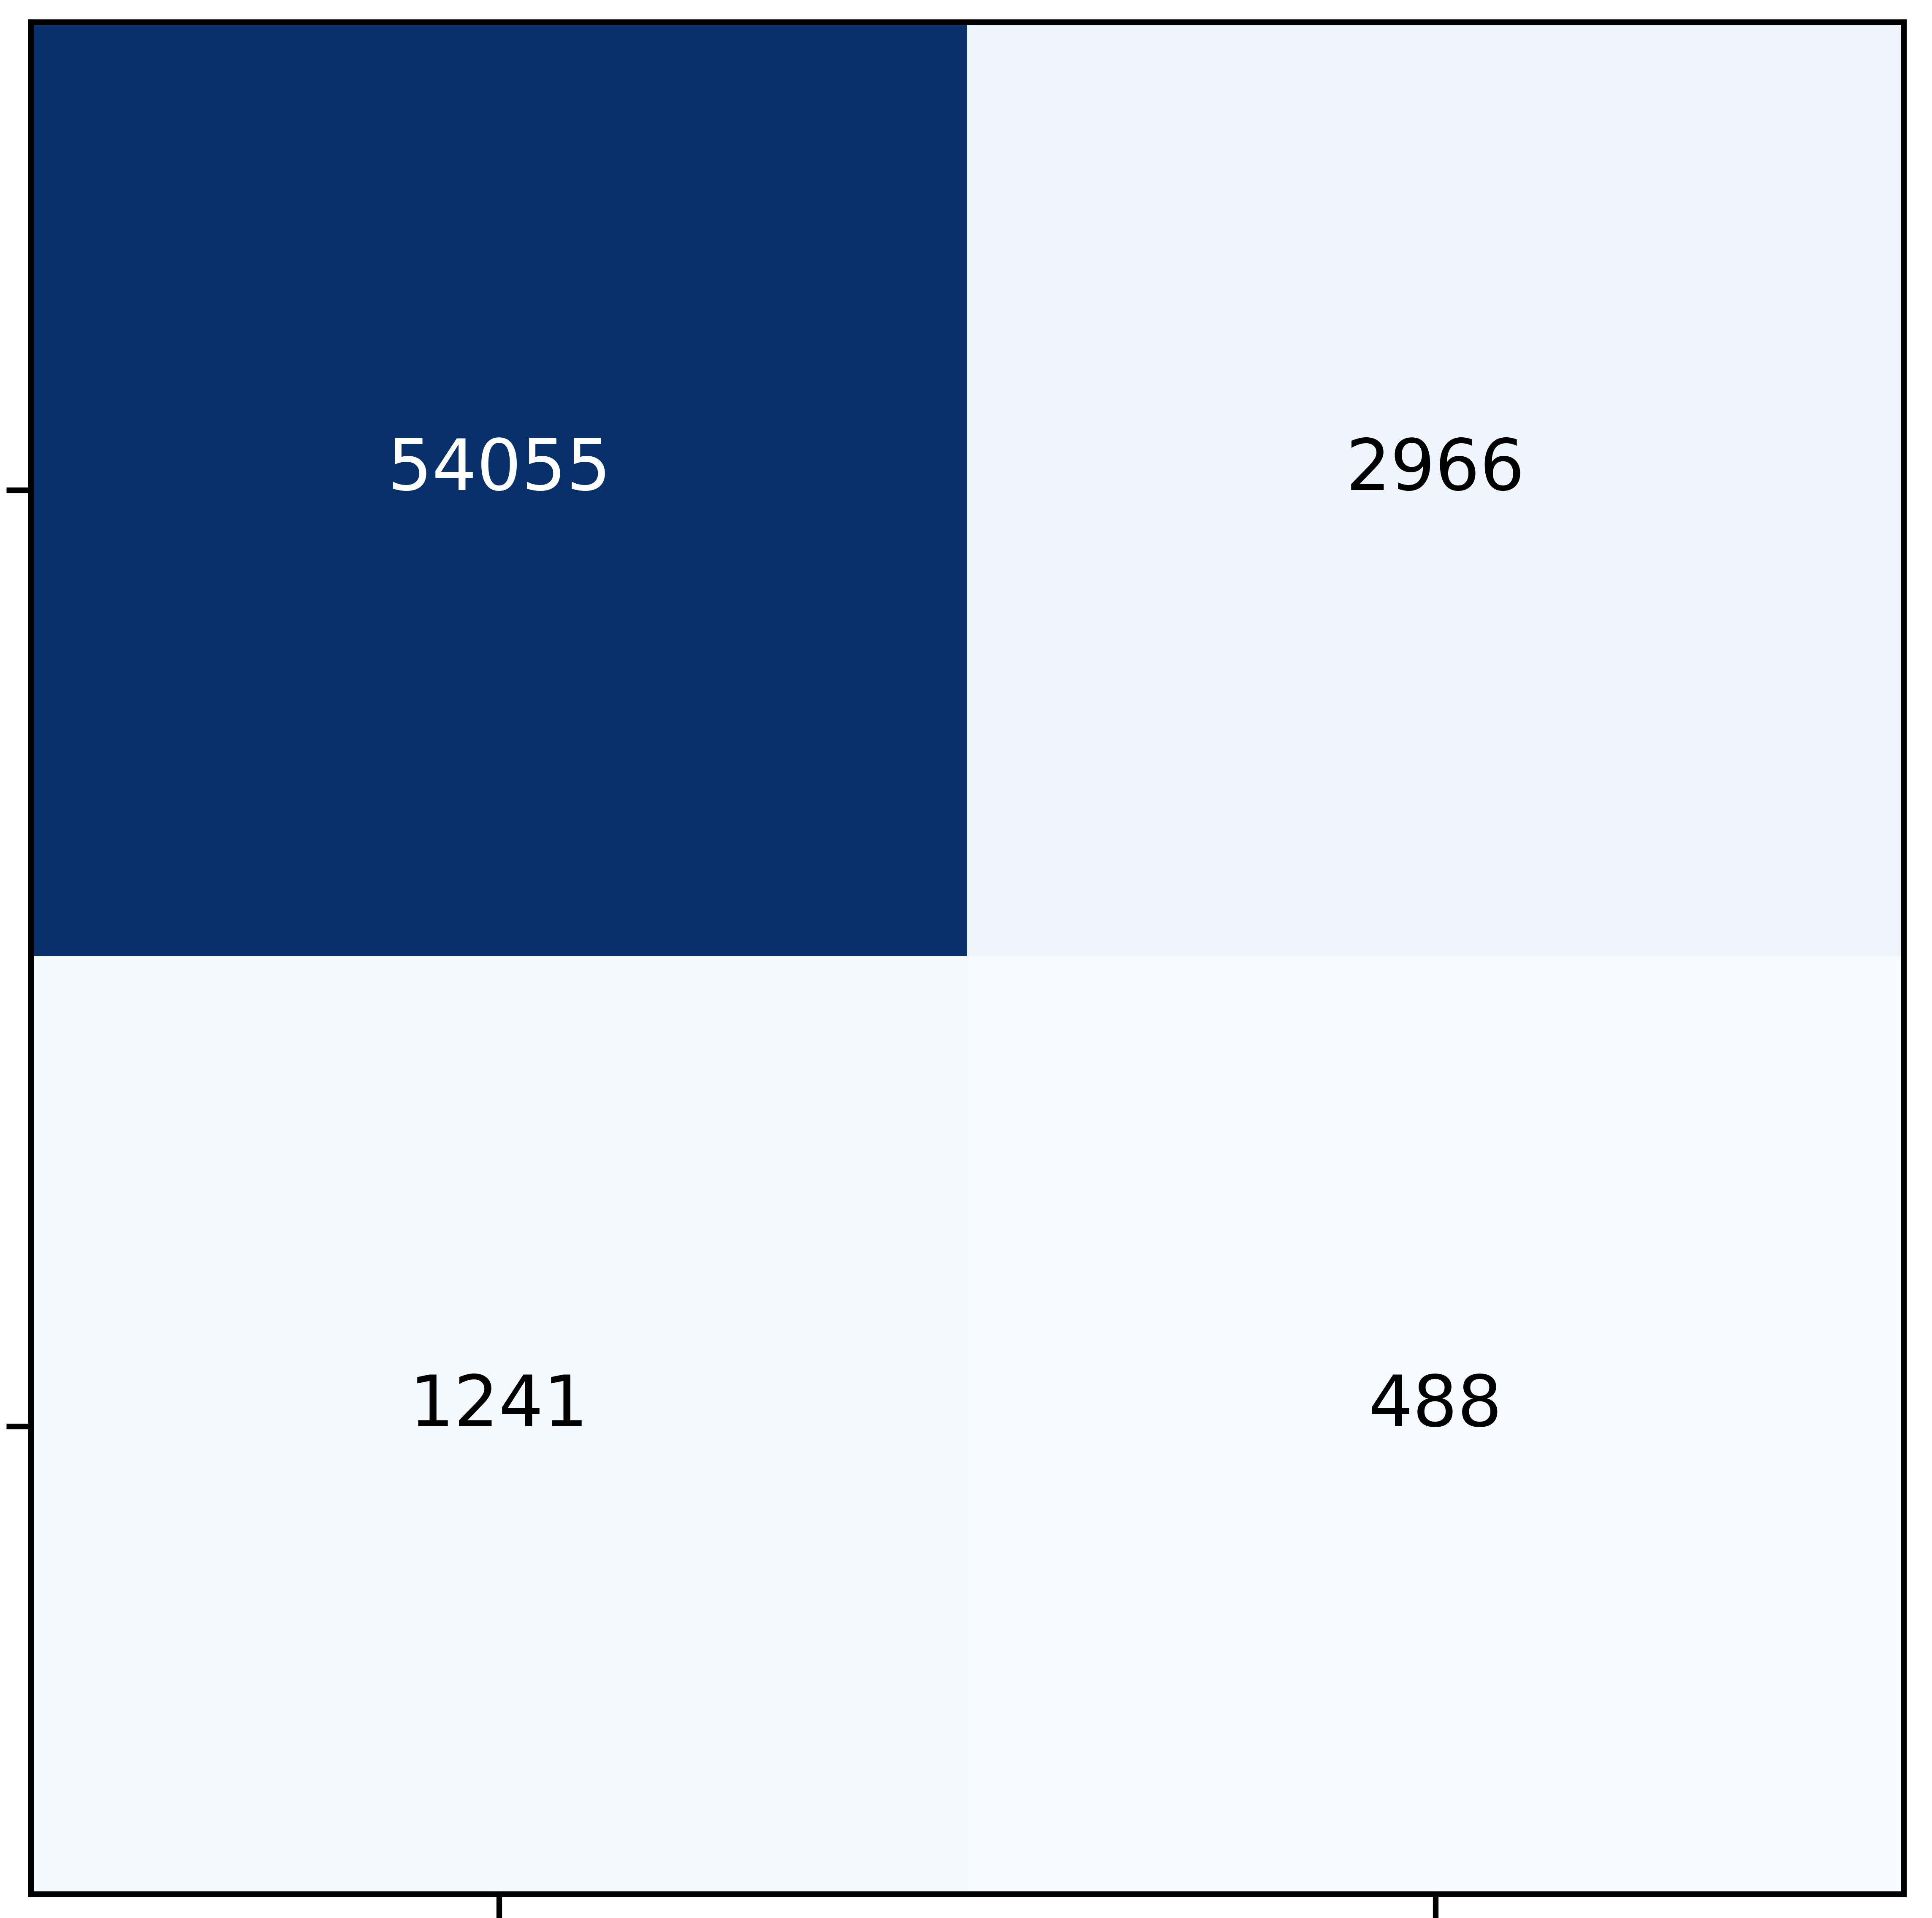
\includegraphics[width=0.478\textwidth]{images/BestConfusionCrop}}
	\end{tabular}
	\caption{Classification of Section 2 using HoG and Gradient Boosting}
	\label{fig:res_best}
\end{figure}

Figure \ref{fig:res_best} shows the most best classification we could achieve using our features sets and classifiers. The results are produced by the experiment described in the experimental setup. For this specific classifcation was performed using the second section with the HoG features, the scales 50, 100 and 150 and Gradient Boosting. This resulted in a F1-Score of 0.19 and a Matthews Coefficient of 0.17. The confusion matrix in the same figure displays the number of correct and incorrect classifications. 

\subsection{Feature Performance}

\pgfplotstableread[col sep = comma]{results/features_sections.csv}\datazero

\begin{figure}
	\begin{tikzpicture}
	\begin{axis}[
	ybar,
	ymajorgrids = true,
	bar width=0.5cm,
	ylabel = Matthews Coefficient,
	width=\textwidth,
	height=.5\textwidth,
	enlarge x limits=0.25,
	symbolic x coords={Section 1, Section 2, Section 3},
	xtick=data,
	ymax = 1,
	yticklabel style={
		/pgf/number format/fixed,
		/pgf/number format/precision=2,
		/pgf/number format/fixed zerofill
	},
	scaled y ticks=false,
	legend columns=4, 
	legend style={
		% the /tikz/ prefix is necessary here...
		% otherwise, it might end-up with `/pgfplots/column 2`
		% which is not what we want. compare pgfmanual.pdf
		/tikz/column 2/.style={
			column sep=5pt,
		},
		at={(0.75, -0.15)},
	}
	]
	\addplot table[x=TestImage, y=HoG]{\datazero};
	\addplot table[x=TestImage, y=LSR]{\datazero};
	\addplot table[x=TestImage, y=RID]{\datazero};
	\addplot table[x=TestImage, y=All features]{\datazero};
	%\addplot[dotted, sharp plot, update limits=false] coordinates {(0, 0)(1, 0)}; 
	\legend{HoG, LSR, RID, All features}
	\end{axis}
	
	\end{tikzpicture}
	\caption{The performance of features measured by Matthews Coefficient}
	\label{fig:res_bar_0}
\end{figure}

The bar plot in Figure \ref{fig:res_bar_0} show the classification performance for the four feature sets on the three sections. To reduce complexity, we only display the results of the classifier with the highest performance instead of all classifiers. Furthermore, we only display Matthews Coefficient because, in many experiments, both values would be very similar.
It seems that HoG performs well for all three sections. LSR is more variable between the three sections. In the second section, LSR is close to HoG in performance, but in section three, it really underperformed. RID seems reasonable in the first section but it has very low performance for the other two sections. The combination of all features seems to perform well, although it is not better than HoG in any section.

\subsection{Classifier Performance}

Although Figure \ref{fig:res_bar_0} shows the maximum performance of the features, it does not display the individual performance of the classifiers. We therefore compare the classification algorithms side by side to gain more insight in the performance differences of the classification algorithms. This comparison is displayed in Figure \ref{fig:res_bar_1}. The bar plot displays the maximum performance that a classifier has obtained for any feature set or test image. To measure performance, we used the maximum of Matthews Coefficient and the F1-Score. It turned out that, for all classifiers, the set of parameters that produced the maximum of Matthews Coefficient was the same set of parameters with the maximum F1-score. That the measurements by two different algorithms is similar suggests that the measure of performance is consistent.

\pgfplotstableread[col sep = comma]{results/classifiers.csv}\dataone

\begin{figure}
	\begin{tikzpicture}
		\begin{axis}[
			ybar,
			bar width=.5cm,
			width=\textwidth,
			height=.5\textwidth,
			ymajorgrids = true,
			legend pos = north west,
			ylabel= Maximum Performance,
			symbolic x coords={DecisionTree, RandomForrest,AdaBoost,GradientBoost,MLP},
			xtick=data,
			yticklabel style={
				/pgf/number format/fixed,
				/pgf/number format/precision=2,
				/pgf/number format/fixed zerofill
			},
			scaled y ticks=false,
		]
		\addplot table[x=Classifier,y=F1-Score]{\dataone};
		\addplot table[x=Classifier,y=Matthews]{\dataone};
	
	
		\legend{F1-Score, Matthews Coefficient}
		\end{axis}
		
	\end{tikzpicture}
	\caption{Maximum Performance of the Classification Algorithms for all sections}
	\label{fig:res_bar_1}
\end{figure}

Figure \ref{fig:res_bar_1} shows that Gradient Boosting was able to produce the best results. The Decision Tree and Random Forrest had the lowest maximum performance. Because this is the maximum performance it does not necessarily follow that this level of performance is also achieved for other parameters as well. We will not investigate the difference in performance between classification algorithm for certain data and parameters any further since this is out of the scope of our thesis.

\subsection{Effect of different Scales}

As we have discussed in the feature evaluation, we suspect increased scale to have a positive effect on the classification performance of the features. In this experiment, the only variable is the different scales. The all other parameters are fixed. We use a single feature set containing all features and section 2 as the test image. This setup was chosen because it has shown to produced good results in the previous experiments, as displayed in Figure \ref{fig:res_bar_0}. The Matthews coefficient on the y axis is scaled up to display the difference in performance more clearly.

\begin{figure}
	\centering
	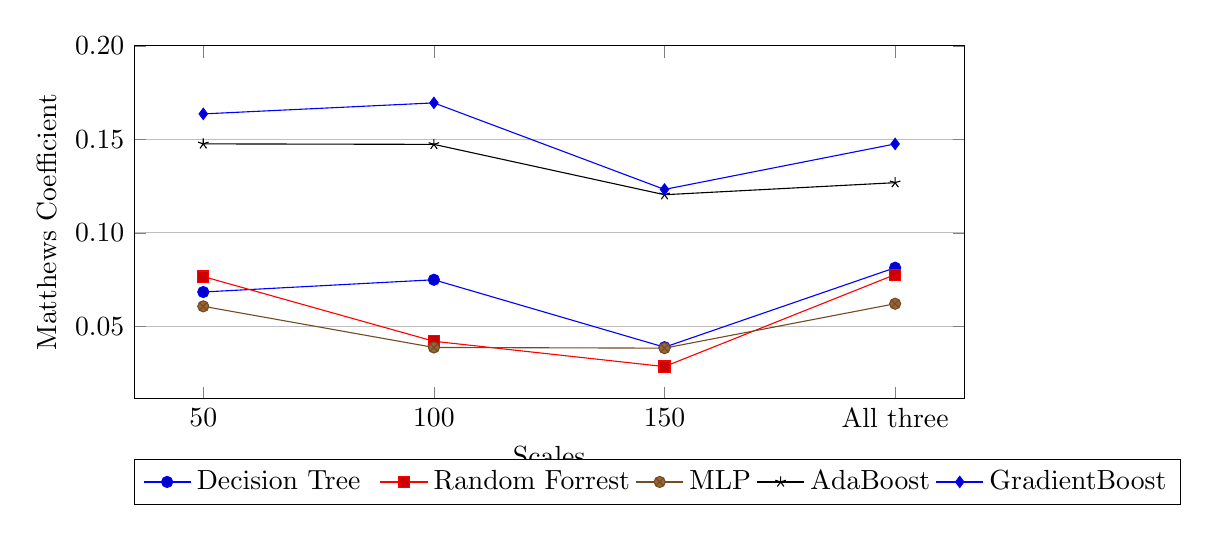
\begin{tikzpicture}
	\begin{axis}[
		title={},
		xlabel={Scales},
		ylabel={Matthews Coefficient},
		width=\textwidth,
		height=.5\textwidth,
		symbolic x coords={50, 100, 150, All three},
		xtick=data,
		ytick={-0.05, 0.0, 0.05, 0.10, 0.15, 0.20},
		yticklabel style={
					/pgf/number format/fixed,
					/pgf/number format/precision=2,
					/pgf/number format/fixed zerofill
				},
		ymax=0.20,
		legend pos=north west,
		ymajorgrids=true,
		legend columns=5, 
		legend style={
			% the /tikz/ prefix is necessary here...
			% otherwise, it might end-up with `/pgfplots/column 2`
			% which is not what we want. compare pgfmanual.pdf
			/tikz/column 2/.style={
				column sep=5pt,
			},
			at={(0.0, -0.17)},
		}
		]
	
		\addplot
		coordinates {
			(50,0.068427407212623)(100, 0.074966895103175)(150, 0.038928267316005)(All three, 0.081409428624833)
		};
		
		\addplot
		coordinates {
			(50, 0.076677199288863)(100, 0.042099627073353)(150, 0.028570812585408)(All three, 0.077733110578942)
		};
		
		\addplot
		coordinates {
			(50,0.060778260530553)(100, 0.038786124761983)(150, 0.038425470626755)(All three, 0.062153606915537)
		};
		\addplot
		coordinates {
			(50, 0.147590307870466)(100,0.147328964006612)(150, 0.120414247378828)(All three, 0.126851482904826)
		};
		\addplot
		coordinates {
			(50, 0.163610733799053 )(100, 0.169491852975136)(150, 0.123248189675469)(All three, 
			0.147566516221729)
		};
		\legend{Decision Tree, Random Forrest, MLP, AdaBoost, GradientBoost}
		
	
	\end{axis}
	\end{tikzpicture}
	\caption{Effects of increased scale for all features on Section 2 as test image}
	\label{fig:res_plot_0}
\end{figure}

The results in Figure \ref{fig:res_plot_0} seem to indicate that increased scale does not necessarily results in improved performance. However, the same experiment, run with Section 1 as test image, did see a slight improvement of performance.

\subsection{Effect of different Block sizes}
% TODO: do on section 1, 2, 3 for scales (50, 100, 150) for (all featatures)




\subsection{Effects of oversampling}
As hinted earlier, oversampling is an important part in classification. Without oversampling, the classifiers are likely to produce trivial results. Oversampling is a common method to balance a dataset. In this section, we evaluate three different oversampling methods. These are random oversampling, SMOTE and ADASYN. The first method randomly picks entries of the minority class and copies these. The last two methods create new synthetic examples that suit the data well.
%TODO: extend


